\documentclass[dvipsnames]{beamer}
\usepackage{lmodern}
\usepackage{appendixnumberbeamer}
\renewcommand{\sfdefault}{lmss}
\renewcommand{\ttdefault}{lmtt}
\usepackage[T1]{fontenc}
% \usepackage[utf8]{inputenc}
\setcounter{secnumdepth}{3}
\setcounter{tocdepth}{3}
\usepackage{amsmath}
\usepackage{amsthm}
\usepackage{amssymb}
\theoremstyle{definition}
\newtheorem*{defn*}{\protect\definitionname}
\providecommand{\definitionname}{Definition}
\usepackage{graphicx}
\usepackage{hyperref}
\usepackage{ulem}
\PassOptionsToPackage{normalem}{ulem}
\usepackage{caption}
\usepackage{subcaption}
\usepackage{verbatim}
\usepackage[english]{babel}
\usepackage[autostyle]{csquotes}
\usepackage{tikz}
\usetikzlibrary{arrows,intersections}
\usepackage{pgfplots}
\pgfplotsset{compat = 1.15}
\usepgfplotslibrary{fillbetween}
\usepackage{verbatim}
\usepackage{booktabs}
\usepackage{multirow}
\usepackage{array}
\usepackage{nccmath}
% \usepackage{listings}
\usepackage{mathtools}

%Bibliography style, etc.
\usepackage[citestyle=authoryear-comp,natbib, uniquename = false, url = false, doi = false, uniquelist=false]{biblatex}
\renewbibmacro{in:}{}
\AtEveryBibitem{%
  \clearfield{volume}%
  \clearfield{number}
  \clearfield{month}
  \clearfield{issn}
  \clearfield{isbn}
  \clearfield{pages}
}

%\usepackage{cleveref}
\usepackage{setspace}
\makeatletter

% Macros
\providecommand{\tabularnewline}{\\}
\newcommand{\gr}{\textcolor{ForestGreen}} 
\newcommand{\rd}{\textcolor{red}}
\newcommand{\cb}{\textcolor{CornflowerBlue}} %this is the blue color you like; simply type \cb{X} where "X" is the color you want in blue
\newcommand{\vitem}{\vfill \item} %auto-centers items in lists
\newcommand{\fall}{\ \forall} %redefines "forall" (I don't like the default spacing)
\newcommand{\frall}{\quad \forall} %a \forall separated from the main math; this is the way it usually shows up in equations
\newcommand{\exist}{\ \exists} %same as \fall, but for \exists; they have the same ugly spacing
\newcommand{\R}{\mathbb{R}} %set of real numbers
\newcommand*\bigcdot{\mathpalette\bigcdot@{.5}} %different size for cdots
% \newcommand{\argmax}{\text{arg}\max}
\newenvironment{itemframe}
    {\frame{}\itemize}
    {\itemize\frame}
\newcommand\makebeamertitle{\frame{\maketitle}}%
\newtheoremstyle{named}{}{}{\itshape}{}{\bfseries}{.}{.5em}{\thmnote{#3's }#1}
\theoremstyle{named}
\newtheorem*{prop*}{Proposition}
% \newtheorem*{corollary}{Corollary}
\newtheorem*{namedtheorem}{Theorem} %allows named theorems
\newtheorem*{nameddef}{Definition}
\newtheorem{proposition}{Proposition}
\newtheorem*{assumption}{Assumption}
\newtheorem*{namedcorollary}{Corollary}
\newtheorem*{namedlemma}{Lemma}
\newtheorem*{axiom}{Axiom}
\newtheorem*{theorem*}{Theorem}
\newtheorem*{lemma*}{Lemma}
\DeclareMathOperator*{\argmin}{argmin}
\DeclareMathOperator{\argmax}{argmax}
\DeclareMathOperator{\supp}{supp}
\DeclareMathOperator{\interior}{int}
\DeclareMathOperator{\rank}{rank}
\newcolumntype{C}[1]{>{\centering\let\newline\\\arraybackslash\hspace{0pt}}m{#1}}
\newcommand{\sbt}{\,\begin{picture}(-1,1)(-1,-3)\circle*{2}\end{picture}\ }



%formatting
\usetheme{Ilmenau}
\definecolor{MIT}{rgb}{.639,.122,.204}
\definecolor{UCLA}{rgb}{0.15294117647058825, 0.4549019607843137, 0.6823529411764706}
\definecolor{UCLA_gold}{rgb}{1, 0.8196078431372549, 0}
\usecolortheme[named=UCLA]{structure}
\setbeamercolor*{palette secondary}{fg=UCLA_gold,bg=gray!15!white}
\usecolortheme{dolphin}
\setbeamertemplate{navigation symbols}{} 
\setbeamertemplate{footline}{}{}
\setbeamertemplate{headline}{}
\setbeamertemplate{navigation symbols}{}
\mode<presentation> {}
\setbeamercolor{block title}{use=structure,fg=white,bg=RoyalBlue} %blocks (theorems, etc.)in blue
\setbeamercolor{block title alerted}{use=structure,fg=white,bg=ForestGreen} %blocks (theorems, etc.)in blue

\renewcommand\qedsymbol{$\blacksquare$} %set QED symbol as black square
\renewcommand{\emph}{\textit} %set emphasized text style; this is italics
\setbeamertemplate{footline}[frame number] %slide numbers
\setbeamertemplate{itemize item}[circle] %bullet style
\setbeamertemplate{itemize subitem}{--}
\setbeamertemplate{enumerate item}[default]
\newrobustcmd*{\parentexttrack}[1]{%
  \begingroup
  \blx@blxinit
  \blx@setsfcodes
  \blx@bibopenparen#1\blx@bibcloseparen
  \endgroup}

\AtEveryCite{%
  \let\parentext=\parentexttrack%
  \let\bibopenparen=\bibopenbracket%
  \let\bibcloseparen=\bibclosebracket}

 \AtBeginDocument{%
   \let\origtableofcontents=\tableofcontents
   \def\tableofcontents{\@ifnextchar[{\origtableofcontents}{\gobbletableofcontents}}
   \def\gobbletableofcontents#1{\origtableofcontents}
 }
\newcommand{\backupbegin}{
   \newcounter{framenumberappendix}
   \setcounter{framenumberappendix}{\value{framenumber}}
}
\newcommand{\backupend}{
   \addtocounter{framenumberappendix}{-\value{framenumber}}
   \addtocounter{framenumber}{\value{framenumberappendix}} 
} 

\renewcommand{\maketitle}{
\setbeamertemplate{footline}{} 
\begin{frame}[noframenumbering]
\titlepage
\end{frame}
\setbeamertemplate{footline}[frame number]
}

\usefonttheme[onlymath]{serif}

% \usetheme{CambridgeUS}

% \newtheorem{theorem}{Theorem}
% \theoremstyle{claim}
\newtheorem{claim}{Claim}
% \newtheorem{corollary}{Corollary}


\makeatother


%\author{Drew Fudenberg}

\institute[]{}
\usepackage{multirow,array}
\title{Learning to Coordinate: A Study in Retail Gasoline}
\author{Byrne and de Roos, \emph{AER} (2019)}
\date{\today}

\begin{document}
\maketitle
\begin{frame}{Games with Multiple Nash Equilibria}
    \begin{table}
    \setlength{\extrarowheight}{2pt}
    \begin{tabular}{cc|c|c|}
      & \multicolumn{1}{c}{} & \multicolumn{2}{c}{Player $Y$}\\
      & \multicolumn{1}{c}{} & \multicolumn{1}{c}{$A$}  & \multicolumn{1}{c}{$B$} \\\cline{3-4}
      \multirow{2}*{Player $X$}  & $A$ & $(3, 3)$ & $(0,0)$ \\\cline{3-4}
      & $B$ & $(0,0)$ & $(5,5)$ \\\cline{3-4}
    \end{tabular}
  \end{table}
  \begin{itemize}
  \vitem Both $(A, A)$ and $(B, B)$ are Nash equilibria.
    \vitem Both players prefer $(B, B)$, but if they start by playing $(A, A)$ how can they get there? And how long does it take?
    \vitem Most theory is agnostic about these questions (e.g. sunspot equilibria)
  \end{itemize}
\end{frame}
  %
  \begin{frame}{Overview}
    \begin{itemize}
      \item Authors look at gas prices in Perth (Australia) and examine how the firms move from one equilibrium to a ``better'' (for the firms) equilibrium.
    \vitem This paper does \rd{not} model the actual game that gas stations are playing. Entirely descriptive (not structural, not reduced form)
      \vitem \textbf{Results:} Market leader price-setting makes it possible for firms to coordinate their pricing strategies (collusion, but legal) and move to an equilibrium with higher markups.
      \begin{itemize}
      \item This process takes about 3.5 years.
        \item There are important institutional details (granular price monitoring) that make tacit collusion in this setting particularly easy.
      \end{itemize}
    \end{itemize}
  \end{frame}
  %
  \begin{frame}{Data/Setting}
    \begin{itemize}
      \item Data from 2001--2015
    \vitem Four large market participants (22 percent for BP; 16/14/16 percent for Caltex, Woolworths, Coles); remainder are small
      \vitem Firms submit tomorrow's prices at 2PM; these are legally binding, and publicly announced at 2.30PM
      \begin{itemize}
      \vitem Consumers don't really pay attention, but this makes it easy for gas stations to check what others are doing
      \vitem Other than location, gas is a homogeneous good with common shocks.
      \vitem No other shocks to the market during this period.
      \end{itemize}
    \end{itemize}
  \end{frame}
  %
  \begin{frame}{Market Cycles}
    \begin{figure}[htp]
      \centering
      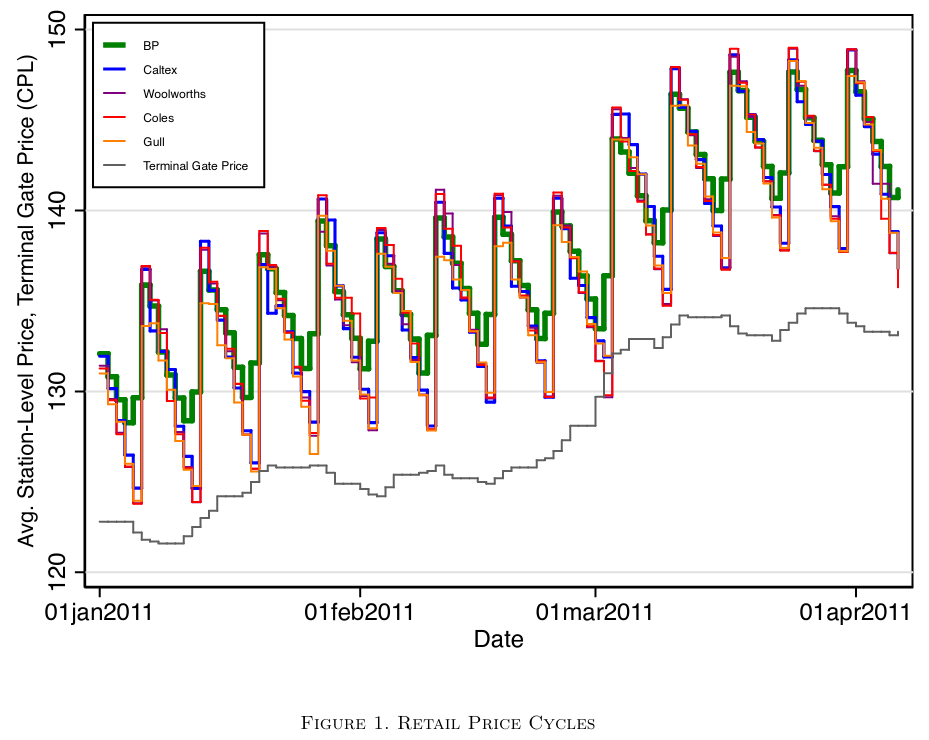
\includegraphics[width=.6\textwidth, keepaspectratio=true]{fig1.png}
    \end{figure}
    \begin{enumerate}
    \item All firms raise prices by the ``same'' amount, on the same day
      \vitem Each day after the price rise (for a set number of days) all firms reduce their prices by the same amount
      \vitem Repeat
    \end{enumerate}
  \end{frame}
  %
  \begin{frame}{First focal point: Thursday jumps}
    \begin{figure}[htp]
      \centering
      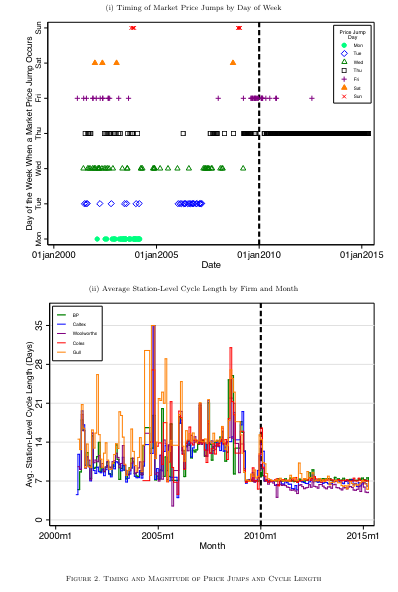
\includegraphics[height=.9\textheight, keepaspectratio=true]{fig2.png}
    \end{figure}
  \end{frame}
  %
  \begin{frame}{Second focal point: 2-cpl cuts}
    \begin{figure}[htp]
      \centering
    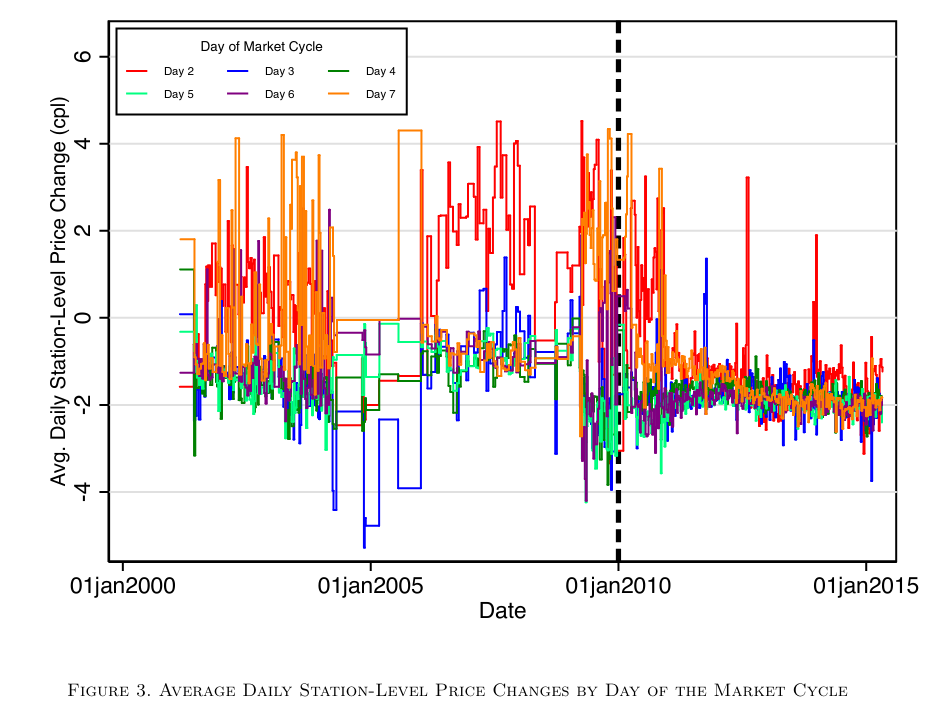
\includegraphics[width=\textwidth, keepaspectratio=true]{fig3.png}  
    \end{figure}
  \end{frame}
  %
  \begin{frame}{What does this mean for firms? Margins grow}
    \begin{figure}[htp]
      \centering
      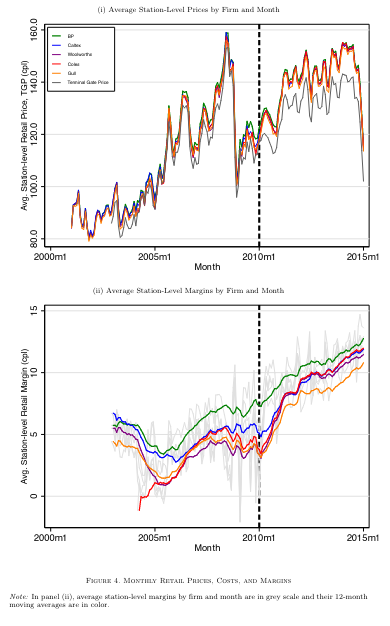
\includegraphics[width=0.55\textheight, keepaspectratio=true]{fig4.png}
    \end{figure}
  \end{frame}
  %
  \begin{frame}{How do firms get to this better equilibrium?}
\begin{columns}
\begin{column}{0.7\textwidth}
    \begin{quote}
      BP is an established price leader\ldots in 2010, with a history of influencing rivals' pricing behavior\ldots firms eventually achieve \ldots price coordination despite having to set their prices simultaneously\ldots
    \end{quote}
\end{column}
\begin{column}{0.5\textwidth}  %%<--- here

      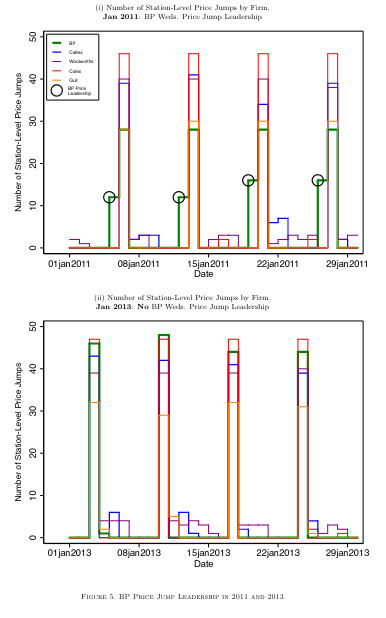
\includegraphics[height=.9\textheight, keepaspectratio=true]{fig5.png}
\end{column}
\end{columns}
  \end{frame}
  %
  \begin{frame}{}
    \begin{figure}[htp]
      \centering
     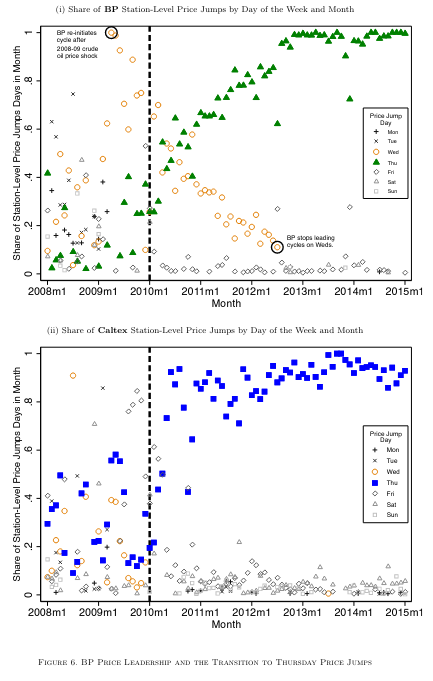
\includegraphics[height=\textheight, keepaspectratio=true]{fig6.png} 
    \end{figure}
  \end{frame}
  %
  \begin{frame}{BP Price Leadership}
    \begin{itemize}
    \item BP randomizes which stations lead price jumps (starting in 2011)
      \vitem Geography isn't important when firms monitor each others' prices (because \emph{all} prices are available online)
      \vitem Randomization allows BP to prevent some stations from getting a reputation for being expensive
    \end{itemize}
  \end{frame}
  %
  \begin{frame}{2-cpl Cuts}
    \begin{figure}[htp]
      \centering
      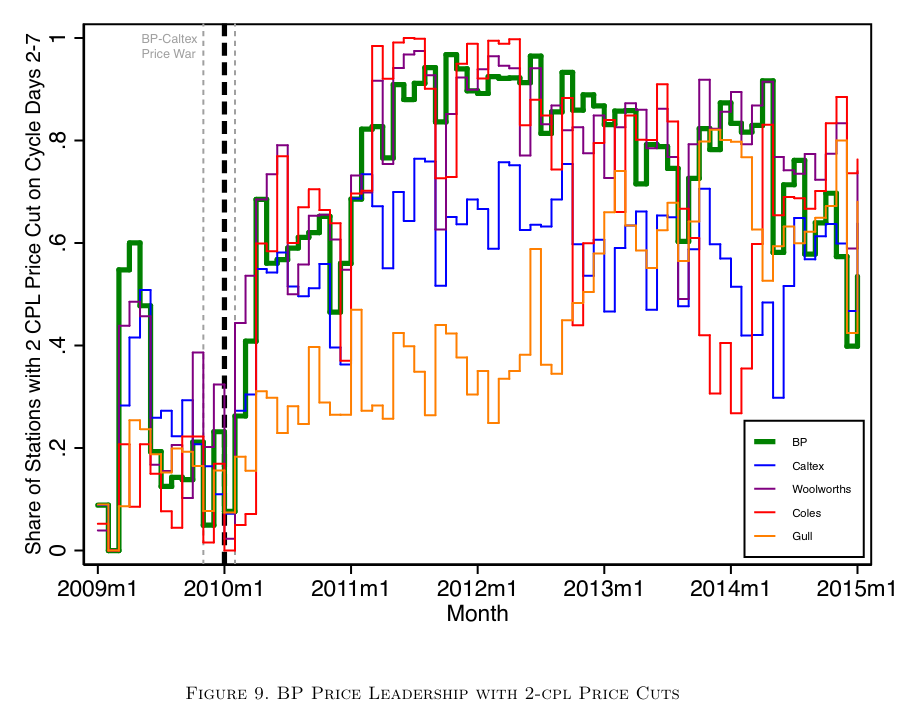
\includegraphics[width=0.8\textwidth, keepaspectratio=true]{fig9.png}
    \end{figure}
    \textbf{Note:} Gull is independent, so ostensibly not colluding with the big firms. 
  \end{frame}
  %
  \begin{frame}{Margin Growth and Coordination}
    \begin{quote}
      BP gradually increases these margins from 14.2-cpl in March 2010 to 17-cpl in July 2012.
    \end{quote}
    \vfill
    \begin{quote}
      How then do firms continue to coordinate on higher Thursday margins over time, absent BP price signaling?
    \end{quote}
    \vfill
    \begin{quote}
      These results point to a self-correcting pricing mechanism whereby firms correct Thursday pricing errors during the undercutting phase of the cycle.
    \end{quote}
  \end{frame}
  %
  \begin{frame}{Price Corrections}
    \begin{columns}
      \begin{column}{0.6\textwidth}
        \begin{quote}
          [F]irms tend to correct overpricing by 2 and 1 cpl above the median on Thursday by cutting prices by 4 and 3 cpl on Friday. That is, if a station overprices on Thursday, their price cut on Friday targets the price level that would have been achieved if the station had matched the median price on Thursday\ldots
        \end{quote}
      \end{column}
      %
      \begin{column}{0.5\textwidth}
        \vspace{-4em}
        \begin{figure}[htp]
          \centering
         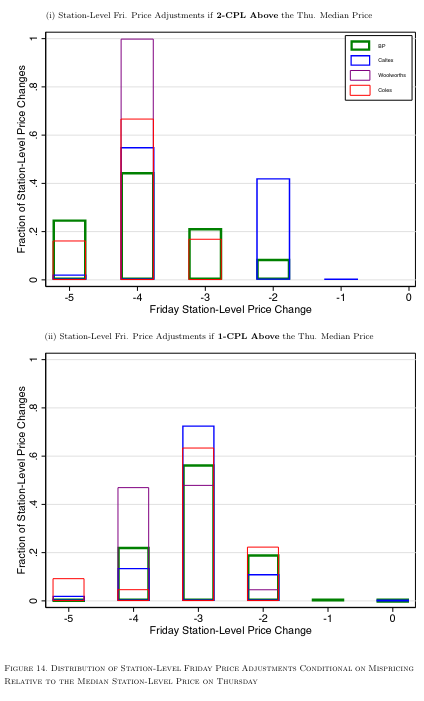
\includegraphics[height=\textheight, keepaspectratio=true]{fig14.png}
        \end{figure}
      \end{column}
    \end{columns}
  \end{frame}
  %
  \begin{frame}{Economic Insights}
    \begin{quote}
     Economists define an equilibrium as collusive if it delivers greater profits than those available in a static Nash equilibrium, and if such profits are supported by punishments off the equilibrium path. How firms start colluding, and how they decide on a particular collusive strategy, is not part of this standard definition. 
    \end{quote}
    \vfill
    \begin{quote}
      While we cannot rule out explicit communication between firms, such as phone calls, the heterogeneous and gradual transition of BP's rivals to a new equilibrium raises concerns of tacit communication by BP through its prices.
    \end{quote}
    \vfill
  \end{frame}
  %
  \begin{frame}{Big picture takeaways}
    \begin{quote}
      Given that firms can perfectly monitor fluctuations in rivals' prices and costs day to day in our setting, it is revealing that BP transitioned the market to a simple pricing structure with Thursday jumps and 2-cpl cuts. This suggests that firms may adopt simple pricing structures, even in the presence of perfect price monitoring, because they are easy to experiment with and communicate to rivals.
    \end{quote}
    \vfill
    \begin{quote}
      As our analysis has shown, long panels are important because profit-enhancing equilibrium transitions can occur over surprisingly long time horizons, three and a half years in our case.
    \end{quote}
    \vfill
  \end{frame}
\end{document}
%%% Local Variables:
%%% mode: latex
%%% TeX-master: t
%%% End:
